%%
%% This is file `sample-sigconf.tex',
%% generated with the docstrip utility.
%%
%% The original source files were:
%%
%% samples.dtx  (with options: `sigconf')
%% 
%% IMPORTANT NOTICE:
%% 
%% For the copyright see the source file.
%% 
%% Any modified versions of this file must be renamed
%% with new filenames distinct from sample-sigconf.tex.
%% 
%% For distribution of the original source see the terms
%% for copying and modification in the file samples.dtx.
%% 
%% This generated file may be distributed as long as the
%% original source files, as listed above, are part of the
%% same distribution. (The sources need not necessarily be
%% in the same archive or directory.)
%%
%%
%% Commands for TeXCount
%TC:macro \cite [option:text,text]
%TC:macro \citep [option:text,text]
%TC:macro \citet [option:text,text]
%TC:envir table 0 1
%TC:envir table* 0 1
%TC:envir tabular [ignore] word
%TC:envir displaymath 0 word
%TC:envir math 0 word
%TC:envir comment 0 0
%%
%%
%% The first command in your LaTeX source must be the \documentclass command.
\documentclass[sigconf]{acmart}

%%
%% \BibTeX command to typeset BibTeX logo in the docs
\AtBeginDocument{%
  \providecommand\BibTeX{{%
    Bib\TeX}}}

%% Rights management information.  This information is sent to you
%% when you complete the rights form.  These commands have SAMPLE
%% values in them; it is your responsibility as an author to replace
%% the commands and values with those provided to you when you
%% complete the rights form.
%%% \setcopyright{acmcopyright}
%%% \copyrightyear{2022}
%%% \acmYear{2022}
%%% \acmDOI{XXXXXXX.XXXXXXX}

%% These commands are for a PROCEEDINGS abstract or paper.
\copyrightyear{2023}
\acmYear{2023}
\setcopyright{acmlicensed}\acmConference[ICIIT 2023]{2023 8th International Conference on Intelligent Information Technology}{February 24--26, 2023}{Da Nang, Vietnam}
\acmBooktitle{2023 8th International Conference on Intelligent Information Technology (ICIIT 2023), February 24--26, 2023, Da Nang, Vietnam}
\acmPrice{15.00}
\acmDOI{10.1145/3591569.3591601}
\acmISBN{978-1-4503-9961-6/23/02}


\usepackage{amsmath}
\usepackage{wrapfig}
%%
%% Submission ID.
%% Use this when submitting an article to a sponsored event. You'll
%% receive a unique submission ID from the organizers
%% of the event, and this ID should be used as the parameter to this command.
%%\acmSubmissionID{123-A56-BU3}

%%
%% For managing citations, it is recommended to use bibliography
%% files in BibTeX format.
%%
%% You can then either use BibTeX with the ACM-Reference-Format style,
%% or BibLaTeX with the acmnumeric or acmauthoryear sytles, that include
%% support for advanced citation of software artefact from the
%% biblatex-software package, also separately available on CTAN.
%%
%% Look at the sample-*-biblatex.tex files for templates showcasing
%% the biblatex styles.
%%

%%
%% The majority of ACM publications use numbered citations and
%% references.  The command \citestyle{authoryear} switches to the
%% "author year" style.
%%
%% If you are preparing content for an event
%% sponsored by ACM SIGGRAPH, you must use the "author year" style of
%% citations and references.
%% Uncommenting
%% the next command will enable that style.
%%\citestyle{acmauthoryear}



%%
%% end of the preamble, start of the body of the document source.

\begin{document}

\title{A Robust and Low Complexity Deep Learning Model \\ for Remote Sensing Image Classification}


\author{Cam Le$^{1,3}$}
\email{cam.levt123@hcmut.edu.vn}
\affiliation{
      \institution{HCMC University of Technology}
      \country{Viet Nam}
}

\author{Lam Pham}
\email{Lam.Pham@ait.ac.at}
\affiliation{
  \institution{Austrian Institute of Technology}
  \country{Austria}
}

\author{Nghia NVN}
\email{nghianguyenbkdn@gmail.com}
\affiliation{
  \institution{Pintel ltd.}
  \country{South Korea}
}

\author{Truong Nguyen$^{2,3}$} % 
\email{truongnguyen@hcmut.edu.vn}
\affiliation{%
  \institution{HCMC University of Technology}
  \country{Viet Nam}
}

\author{Le Hong Trang$^{1,3}$} % 
\email{lhtrang@hcmut.edu.vn}
\affiliation{
  \institution{HCMC University of Technology}
  \country{Viet Nam}
}

\thanks{1. Faculty of Computer Science and Engineering}
\thanks{2. Faculty of Electrical and Electronics Engineering}
\thanks{3. HCMC University of Technology (HCMUT), 268 Ly Thuong Kiet, District 10, Ho Chi Minh City, Viet Nam and Vietnam National University Ho Chi Minh City (VNU-HCM), Linh Trung Ward, Thu Duc City, Ho Chi Minh City, Vietnam.}


\renewcommand{\shortauthors}{Cam Le et al.}

\begin{abstract}
In this paper, we present a robust and low complexity deep learning model for Remote Sensing Image Classification (RSIC), the task of identifying the scene of a remote sensing image.
In particular, we firstly evaluate different low complexity and benchmark deep neural networks: MobileNetV1, MobileNetV2, NASNetMobile, and EfficientNetB0, which present a number of trainable parameters lower than 5 Million (M) or occupy 20 MB memory.
After indicating the best network architecture, we further improve the network performance by applying attention schemes to multiple feature maps extracted from middle layers of the network.
To deal with the issue of increasing the model footprint due to using attention schemes, we apply the quantization technique to satisfy the maximum memory occupation of 20 MB.
By conducting extensive experiments on the benchmark datasets NWPU-RESISC45, we achieve a robust and low-complexity model, which is very competitive to the state-of-the-art systems and potential for real-life applications on edge devices.
\end{abstract}

\begin{CCSXML}
<ccs2012>
  <concept>
      <concept_id>10010147.10010178</concept_id>
      <concept_desc>Computing methodologies~Artificial intelligence</concept_desc>
      <concept_significance>500</concept_significance>
      </concept>
 </ccs2012>
\end{CCSXML}

\ccsdesc[500]{Computing methodologies~Artificial intelligence}

\keywords{Deep learning, convolutional neural network (CNN), remote sensing image classification (RSIC), data augmentation, model complexity.}


\maketitle


\section{INTRODUCTION}
\label{intro}

As the task of remote sensing image classification (RSIC) is considered as an important component in various real-life applications such as urban planning~\cite{thapa2009urban, netzband2007applied}, natural hazards detection~\cite{poursanidis2017remote, van2013remote}, environmental monitoring~\cite{van2013remote}, vegetation mapping or geospatial object detection~\cite{feng2015uav}, it has attracted much research attention in recent years.
Indeed, the research community, which focuses on RSIC tasks, has published diverse datasets of remote sensing images as well as proposed a wide range of classification models.
The most early dataset of remote sensing images, UCM~\cite{yang2010bag}, was published in 2010.
In the next years, various remote sensing image datasets were published such as WHU-RS19~\cite{Xia2010WHURS19} in 2012, NWPU VHR-10~\cite{cheng2014multi}, SAT6~\cite{basu2015deepsat} and RSSCN7~\cite{zou2015deep} in 2015, SIRI-WHU~\cite{zhao2015dirichlet} in 2016, AID~\cite{xia2017aid} and NWPU-RESISC45~\cite{cheng2017remote} in 2017, and OPTIMAL~\cite{wang2018scene} in 2018.
Among these datasets, NWPU-RESISC45~\cite{cheng2017remote} presents the largest number of 45 different image scenes and a balanced number of 700 images per class.
Regarding RSIC systems, they can be separated into two approaches.
The first approach mainly focuses on image processing techniques and machine learning based classification.   
While image processing techniques are used to extract distinct features from the original image data, traditional machine learning methods are used to classify these extracted features into certain classes. 
Regarding image processing based feature extraction, a wide range of methods were proposed such as Texture Descriptors (TD), Color Histogram (CH), Scale-Invariant Feature Transformation (SIFT) \cite{yang2008comparing}, wavelet transformation with Gabor/Haar filters \cite{elmannai2013support, elmannai2016new}, bag-of-visual-words (BoVW) based techniques \cite{yang2010bag, sridharan2014bag}.
These methods make effort to transform the original image into a new and condensed feature space, likely vector, which is suitable for traditional machine learning classification such as  Support Vector Machine (SVM)~\cite{yang2010bag, elmannai2016new}, K-means Clustering~\cite{zheng2008k}, or Decision Tree and Neural Network\cite{du2012multiple}. In the second approach, RSIC research community focuses on deep learning based models, mainly using variants of Deep Convolutional Neural Network (DCNN) such as VGG \cite{ye2021lightweight}, ResNet \cite{shabbir2021satellite}, DenseNet \cite{tong2020channel}, EfficientNet\cite{zhang2020transfer}, or Transformer \cite{zhang2021trs}. To train these networks, there are two typical strategies\cite{nogueira2017towards}: direct training and transfer learning (fine tuning or using deep neural network as a feature extractor). While the first strategy directly trains a network architecture on a RSIC dataset~\cite{pham2022remote}, the transfer learning approach makes use of pre-trained models on large-scale image datasets to finetune~\cite{hu2015transferring, wang2022empirical, shabbir2021satellite} or extract features~\cite{minetto2019hydra, zhao2020remote, li2020augmentation, zhang2021best, li2021gated, pham2022remote} on a RSIC dataset (i.e. Leveraging a pre-trained model is considered as the transfer learning technique).
As most datasets of RSIC present a limitation of data compared with natural image datasets such as ImageNet~\cite{imagenet_dataset}, training a network from scratch shows high cost and presents ineffective compared with the transfer learning approach.

Compare between two approaches, the second approach leveraging deep learning based systems proves robust and outperforms the traditional machine learning based approach~\cite{mehmood2022remote}. 
However, complicated deep neural networks in the second approach commonly present very high model complexity which causes challenges for applying RSIC on edge devices. 
In this paper, we address the problems of those two approaches and aim to develop a robust and low-complexity deep learning model for the RSIC task. We mainly contribute: 

\begin{enumerate}
\item Firstly, we evaluate and compare current benchmark and low-complexity network architectures: MobileNet, MobileNetV2, NASNetMobile, EfficientB0.
Our experimental results indicate that the EfficientNetB0 architecture using the transfer learning technique is more effective for the RSIC task.\\

\item Secondly, we propose a Multihead attention based layer which is applied to multiple feature maps for improving EfficientNetB0 network performance. 
To deal with the issue of increasing model complexity as using the attention layers, we apply the quantization technique to meet the requirement:  The proposed model footprint occupies a maximum of 20 MB memory which is potential for applying to a wide range of edge devices surveyed in \cite{sun2021mind}. \\ 

\item Finally, we evaluate our best model (EfficientNetB0 network architecture using the transfer learning technique, the proposed Multihead attention based layer, and the quantization technique) on the largest and benchmark dataset of NWPU-RESISC45~\cite{cheng2017remote}.  
The experimental results show that our proposed RSIC system is competitive to the state of the art, but presents a significantly lower model footprint. 
\end{enumerate}

\section{Background}

As our proposed deep learning model leverages the parameter-based transfer learning technique and attention schemes, the background of these two techniques is comprehensively presented below.

\subsection{The parameter-based transfer learning applied for deep neural network}
\label{transfer}
Humans can be aware that it is easy to transfer knowledge from one domain or task to another. 
For instance, it will be easier for a person to learn a second programming language if he/she had experience in a programming language before.
In other words, a person can encounter a new task without starting from scratch by leveraging previous experience to learn and adapt to a new task.
Inspired by the human capability to transfer knowledge, the machine learning research community has recently focused on transfer learning techniques and made effort to apply on the computers~\cite{survey_transfer, survey_transfer_02}.
In this paper, we apply the parameter-based transfer learning technique, which is very popular and effective for deep neural network~\cite{pires2019convolutional}. 
Given a model of neural network architecture, we firstly define the term of `pre-trained model': A model was trained on a particular large-scale dataset for a certain task in advance, referred to as the up-stream task.
Then, transfer learning is a term that points out the action of applying the pre-trained model for a new task but related to some aspect of the up-stream task. 
The new task is referred to as the down-stream task.
Commonly, the up-stream task is more challenging than the down-stream task (e.g., more objects in tasks of object detection or more categories in classification tasks) and the dataset used in the down-stream task is normally smaller or more specific than the large-scale and general dataset for the up-stream task. 
The idea and advantages behind the parameter-based transfer learning technique for deep neural network is that utilizing the information gained while solving a challenging up-stream task (i.e. The trainable parameters and the network architecture of the pre-trained model) may not only save time but also enhance the performance on a more simple down-stream task.
Regarding the mathematical perspective behind the classification task and deep neural network based model in this paper, it is basically an optimization task which makes gradient descent find the minimum point.
Therefore, the starting point of gradient descent is a very important factor.
Indeed, if the starting point of the gradient is near the global optimum point, it significantly helps to save the training time as well as avoid the gradient to converse at unexpected local optimization points.
By applying the parameter-based transfer learning technique, the distribution of trainable parameters, which is reused from a pre-trained model on an up-stream task, is likely to be near the golden distribution of trainable parameters in a down-stream task rather than random initialization. 
As the start distribution of trainable parameters is likely the same as the golden distribution of trainable parameters, the gradient is feasible to converse at very near the global optimal point. 

In this paper, we aim to classify remote sensing images into sentiment categories, which is considered as the task of remote sensing image classification (RSIC).
As we leverage the parameter-based transfer learning technique, our task of RSIC is referred to as the down-stream task.
To solve our down-stream task of RSIC, we need to define the up-stream task of image classification as well as indicate a pre-trained model with a large-scale dataset.
As ImageNet is considered as the benchmark dataset~\cite{Imagenet} to evaluate a wide range of network architectures on the task of image classification, published pre-trained models on ImageNet from Keras library~\cite{keras_app} are considered as the up-stream tasks and leveraged for our down-stream task of RSIC.
 

\subsection{Attention schemes in computer vision}
\label{attention}

Humans can easily find the important regions in an image.
In other words, there are some regions on an image containing specific and distinct features which help humans distinguish from other images. 
This inspires the computer vision research community to focus on attention mechanisms which help deep learning models know and learn which valuable features.  
An attention mechanism can be formulated by a function $g(\mathbf{X})$ where $\textbf{X}$ is the input feature map and $g(\mathbf{X})$ represents a way to create the guidance based on the importance of input feature map $\mathbf{X}$.
In other words, the output of $g(\mathbf{X})$ is attention weights which present which region of the input feature map is more important.
The attention weights are then element-wise multiplied with the input feature map $\textbf{X}$~\cite{hu2018squeeze, woo2018cbam} as described by Eq.~\ref{eq:att}
\begin{align}
   \label{eq:att}
   f(\mathbf{X}) = g(\mathbf{X}) \odot \mathbf{X}
\end{align}
where $f(\mathbf{X})$ is the attention layer applied on the input feature map $\mathbf{X}$ to generate a new feature map which better presents distinct features, but still retains the original feature map size.

The current attention mechanisms applied to the computer vision research field and deep learning models can be divided into some main groups described in detail below.

\textbf{Squeeze-and-excitation networks (SE)}~\cite{hu2018squeeze}: It is a channel-based attention mechanism, which focuses on the particular features on the channel dimension. 
Overall, the SE method is formulated by Eq.~\ref{eq:se}.
\begin{align}
   \label{eq:se}
   f_{SE} = g(mlp(GAP(\mathbf{X}))) \odot \mathbf{X}
\end{align}
where ${g()}$ is sigmoid function, $mlp()$ stands for multi-layers perceptron neural network and GAP is a channel wise global average pooling layer.
Initially, a global average pooling (GAP) is applied to the input feature map before feeding into a multi layers perceptron neural network with a sigmoid function at the last layer. 
Then, a channel-wise multiplication between the input feature map $\mathbf{X}$ and the output of the sigmoid activation layer is applied.

\textbf{Channel attention (CA):} CA mechanism is a variant of SE and it is also a channel-based attention method which has been popularly used in convolutional neural networks~\cite{guo2019global, Zhao_2022}. 
Similar to SE, the idea behind the CA is guiding the model to focus on some particular features on the channel, but CA utilizes information from both global max and average pooling layers.
In particular, given three-dimensional input feature map $\mathbf{X}\in R^{W\times H\times C}$ where $W, H,$ and $C$ are width, height, and channel dimensions, the channel attention (CA) applied to the feature map $\mathbf{X}$ can be formulated by:
\begin{align}
   \label{eq:ca}
   f_{CA} = g(mlp(GAP(\mathbf{X})) +  mlp(GMP(\mathbf{X})))  \odot \mathbf{X}
\end{align}
where ${g()}$ is a sigmoid function, $mlp()$ is a sharing neural layer (e.g. normally use multi-layers perceptron). 
GAP and GMP are global average pooling and global max pooling of channel wise, respectively.

\textbf{Spatial attention (SA):} enables the deep neural network to focus on distinct features on both width and height dimensions rather than the channel dimension as CA or SE mechanisms.
As focusing on the spatial features on width and height dimensions, the channel dimension of a three-dimensional input feature maps $\mathbf{X}$ is firstly reduced by using average pooling and max pooling, create two-dimension feature maps of $\mathbf{X_{A}, X_{M}}{\mathnormal{\in R^{W\times H}}}$, respectively.
Then, a network layer (e.g., normally a convolutional layer), described by $conv()$ is applied and followed by a Sigmoid function.
The SA layer is formulated as Eq.~\ref{eq:sam}
\begin{align}
   \label{eq:sam}
   f_{SA} = g(conv( [\mathbf{X_{A}}, \mathbf{X_{M}}] ) ) \odot \mathbf{X}
\end{align}
where $g()$ is sigmoid function, $conv()$ represents for a convolutional layer.
 
\textbf{Convolutional Block Attention Module (CBAM):} While SE/CA and SA mechanisms only focus on either channel features or spatial features, CBAM~\cite{woo2018cbam}, combines both these attention methods, creating a robust guidance for the network to process important regions of a certain feature map.
This attention mechanism can be described by formulas: Eq.\ref{eq:cbam1} and Eq.\ref{eq:cbam2}:
\begin{align}
   \label{eq:cbam1}
   \mathbf{X'} =  f_{CA}(\mathbf{X}) \\
   \label{eq:cbam2}
   f_{CBAM} =  f_{SA}(\mathbf{X'}) 
\end{align}
where $f_{CA}$ and $f_{SA}$ are from Eq.~\ref{eq:ca} and Eq.~\ref{eq:sam}.

\textbf{Multihead self attention (MSA):} Unlike above methods which make effort to enhance important regions of a feature map, this attention scheme \cite{vaswani2017attention} helps to indicate the similarity score, the dependency between regions in the feature map.
In other words, Multihead self attention is effective to represent the relation between two regions of a feature map which are closed or far from each other. 
Regarding the mathematical intuition behind the Multihead self attention, each attention head can be described as mapping a query ($\mathbf{Q}$) and a set of key($\mathbf{K}$)-value($\mathbf{V}$) pairs to an output, where $\mathbf{Q}$, $\mathbf{K}$, $\mathbf{V}$ obtained through a linear transformation of the input feature map $\mathbf{X}$ as shown in Eq. \ref{eq:mha_q}, Eq. \ref{eq:mha_k}, and Eq. \ref{eq:mha_v}.
\begin{align}
   \label{eq:mha_q}
   \mathbf{Q} =  \mathbf{X} \cdot \mathbf{W_{q}} \\
   \label{eq:mha_k}
   \mathbf{K} =  \mathbf{X} \cdot \mathbf{W_{k}} \\
   \label{eq:mha_v}
   \mathbf{V} =  \mathbf{X} \cdot \mathbf{W_{v}} 
\end{align}
where  $\mathbf{W_{q}, W_{k}, W_{v}}$ are weight matrices.
Then, the output of an attention head can be calculated using Eq.~\ref{eq:one_head}. 
\begin{align}
   g_{n} =  softmax(\frac{\mathbf{Q}\mathbf{K^{T}}}{\sqrt{\mathbf{d_{k}}}})\mathbf{V} 
  \label{eq:one_head}
\end{align}
where $g_{n}$ is the $n^{th}$ attention head,$\mathbf{K^{T}}$ is the transpose of $\mathbf{K}$ and $\mathbf{d_{k}}$ is the number of key dimension which is one of the dimensions of the weight matrices $\mathbf{W_{q}, W_{k}, W_{v}}$.

As each attention head learns a different set of weight matrices $\mathbf{W_{q}, W_{k}, W_{v}}$, they will be different from each others. 
Therefore, when joining many self attention heads together followed by a linear transformation or an addition operation as an ensemble of multiple heads, it forms a Multihead self attention layer which helps to learn an input feature map better.
A Multihead self attention layer with $N$ heads which is applied on the input feature map $\mathbf{X}$ is described by
\begin{align}
    \label{eq:mha_head}
     f_{MA}=  \sum_{n=1}^{N} g_{n}   \odot \mathbf{X}
\end{align}

\section{Proposed deep learning based system for RSIC task}
\label{framework}

Overall, the high-level architecture of our proposed deep learning based system for RSIC task is presented in Figure~\ref{fig:CAM_high}. 
As Figure~\ref{fig:CAM_high} shows, the proposed RSIC system is separated into two main parts: data augmentation and a deep neural network for classification.

\subsection{Data augmentation methods}
\label{augmentation}

In this paper, we apply five data augmentation methods: Image Rotation (IR)~\cite{rotation_aug}, Random Cropping (RC)~\cite{rotation_aug}, Random Erasing (RE)~\cite{spec_crop}, Random Noise Addition (RNA), and Mixup (Mi)~\cite{mixup1, mixup2} to the remote sensing image input data.
As Random Cropping (RC)~\cite{rotation_aug}, Random Erasing (RE)~\cite{spec_crop}, Random Noise Addition (RNA), and Mixup (Mi)~\cite{mixup1, mixup2} are used on batches of images during the training process, they are referred to as the online data augmentation methods. 
Meanwhile, Image Rotation (IR)~\cite{rotation_aug} is referred to as the offline data augmentation as this method is applied on the original dataset before the training process.

Initially, all images in the original dataset are rotated using three different angles: 90, 180, and 270, respectively.
This data augmentation method is referred to as Image Rotation (IR) and an example of IR method with an angle of 90 degree is shown in Figure~\ref{fig:CAM_aug} (b).
As three angles mentioned are used, we obtain a new dataset which is four times larger than the original dataset (i.e. the original images and three new images generated by Image Rotation method with three angles).
\begin{figure}[t]
    \centering
    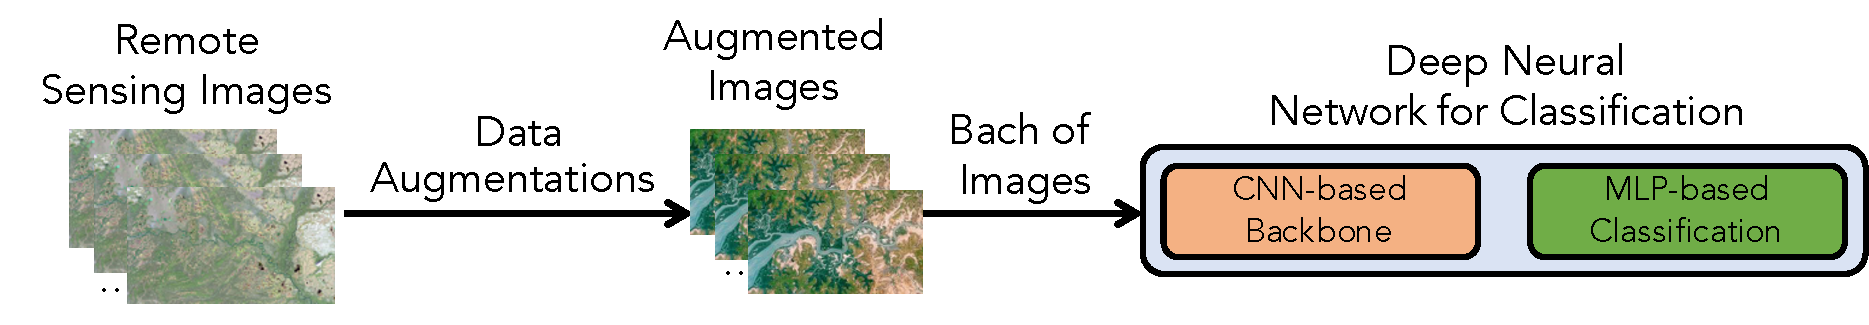
\includegraphics[width=1.0\linewidth]{CAM_high.pdf}
	\caption{The high level architecture of proposed RSIC system}
    \label{fig:CAM_high}
\end{figure}
Next, batches of 60 images are randomly selected from the new dataset.  
For each batch, we apply Random Cropping (RC)~\cite{rotation_aug}, Random Erasing (RE)~\cite{spec_crop}, Random Noise Addition (RNA), and Mixup (Mi)~\cite{mixup1, mixup2} methods, respectively.
Firstly, images in a batch are randomly cropped with a reduction of 10 pixels on both of width and height dimensions as shown in Figure~\ref{fig:CAM_aug} (c) (i.e., The channel dimension is retained), referred to as Random Cropping (RC).
Next, on both width and height dimensions of each image, 20 random and continuous pixels are erased as shown in Figure~\ref{fig:CAM_aug} (d), referred to as Random Erasing (RE). 
The cropped and erased images are then added by a random noise which is generated from Gaussian distribution as shown in Figure~\ref{fig:CAM_aug} (e), referred to as Random Noise Addition (RNA). 
Finally, the images are mixed together with random ratios as shown in Figure~\ref{fig:CAM_aug} (f), referred to as Mixup (Mi).
As both Uniform and Beta distributions are used to generate the mixup ratios as well as we use both the original image and the new mixup images, the batch size increases three times from 60 to 180 images.
\begin{figure}[t]
    \centering
    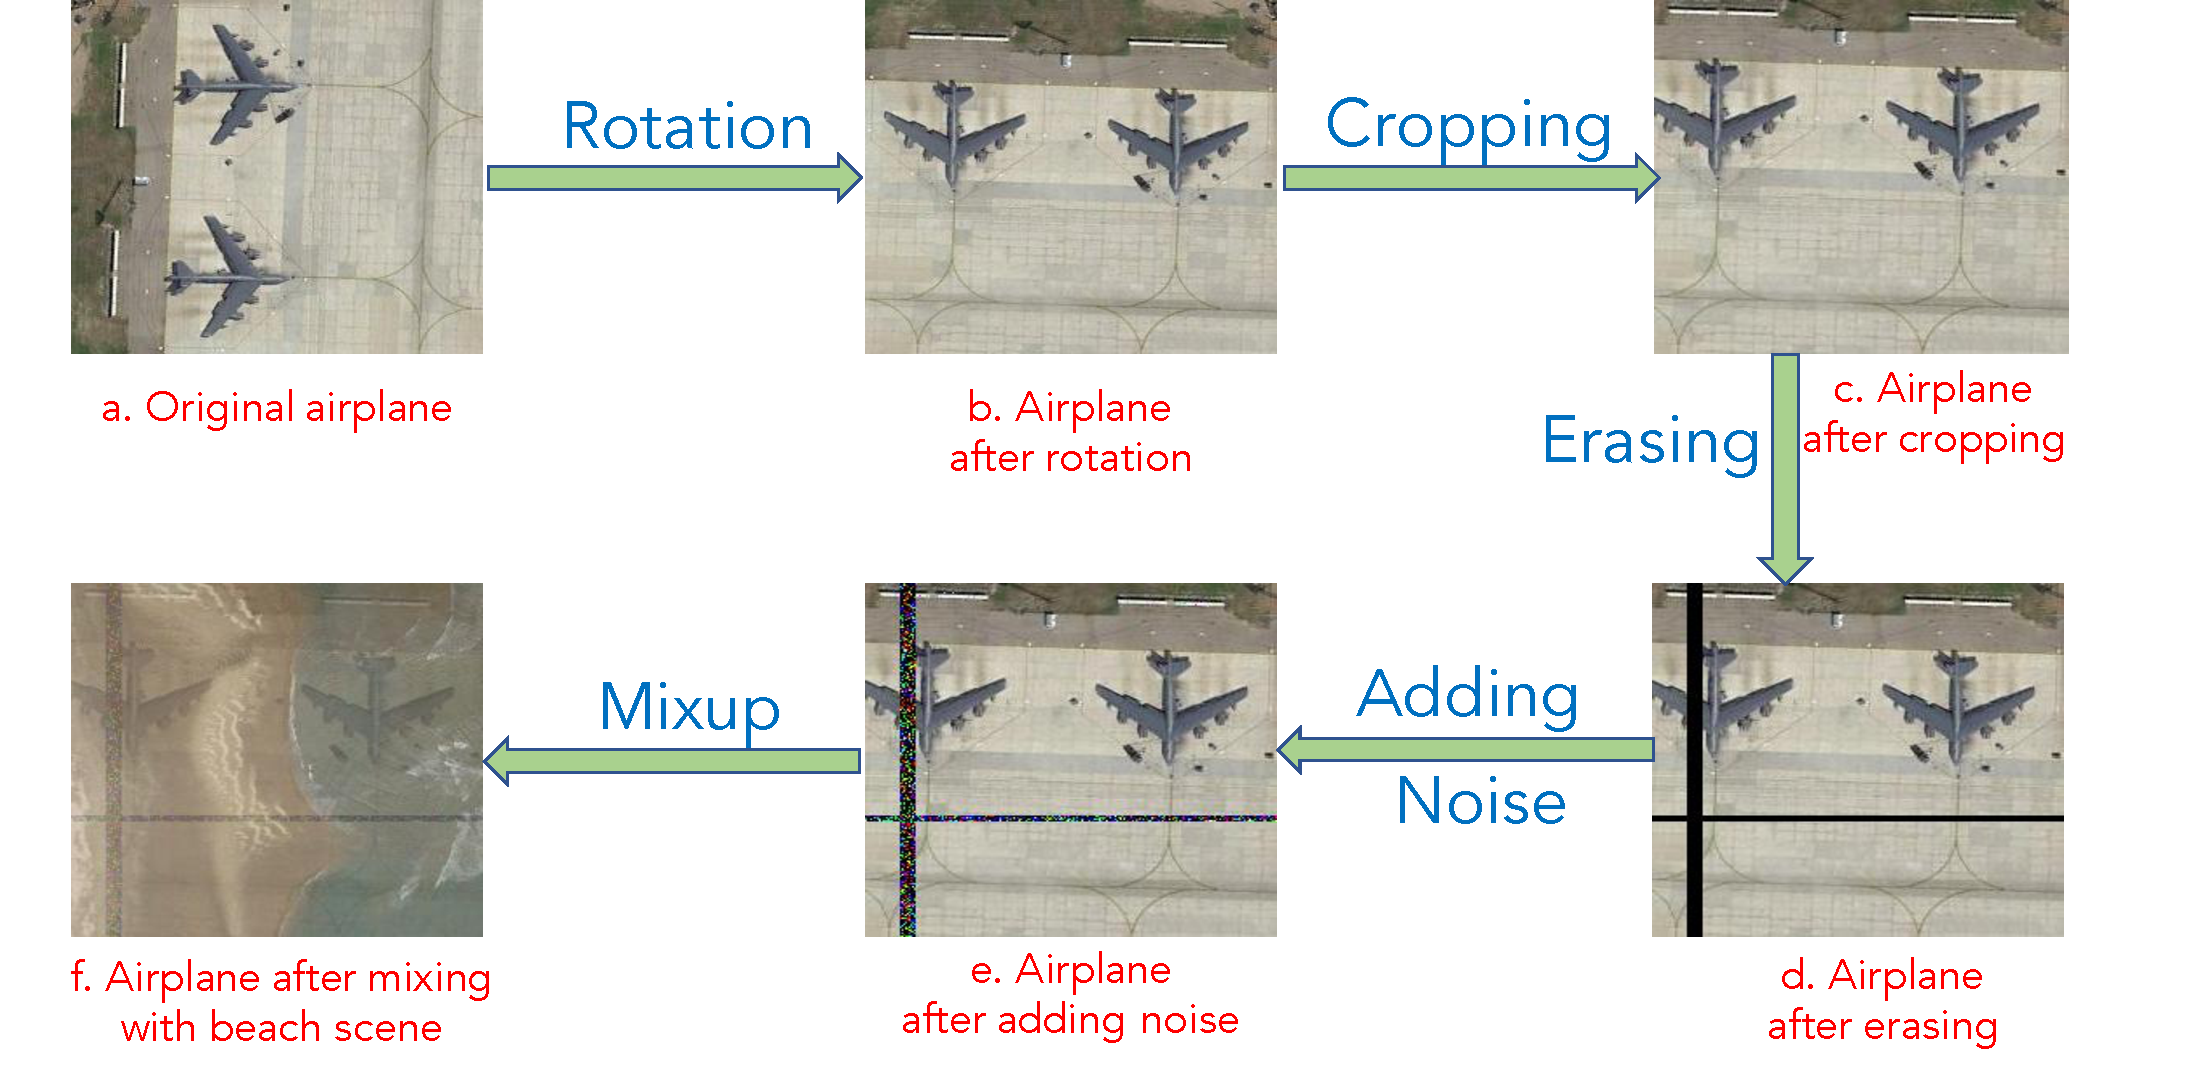
\includegraphics[width=1.0\linewidth]{CAM_aug.pdf}
	\caption{Data augmentation methods: Rotation, Random Cropping, Random Erasing, Adding Noise, and Mixup in the order.}
    \label{fig:CAM_aug}
\end{figure}

\subsection{Apply the transfer learning technique for our proposed deep neural network classification}
\label{neural}

As Figure~\ref{fig:CAM_high} shows, our proposed deep learning model for classification can be separated into two main parts: The convolutional neural network based backbone (CNN based backbone) and the multilayer perceptron based classification (MLP-based classification).
While the CNN based backbone helps to transfer the input images to condensed feature maps, the MLP based classification classifies these condensed feature maps into certain categories.

To indicate which CNN based backbone is effective for RSIC task, we evaluate different benchmark deep neural network architectures which are available in Keras library~\cite{keras_app}.
As we aim to achieve a low-complexity model for RSIC which is lower than 5 M of trainable parameters or occupy less than 20 MB memory (i.e. 1 trainable parameter is presented by 32 bits in floating point format), only four network architectures of MobileNetV1, MobileNetV2, NASNetMobile, and EfficientNetB0 from Keras library~\cite{keras_app} are evaluated.
To leverage these network architectures, we apply the parameter-based transfer learning technique which is mentioned in Section~\ref{transfer}.
The transfer learning process is mainly described in Figure~\ref{fig:CAM_transfer}.
In particular, the benchmark networks of MobileNetV1, MobileNetV2, NASNetMobile, and EfficientNetB0 as described in the higher part of Figure~\ref{fig:CAM_transfer} are firstly trained with the large scale dataset of ImageNet, referred to as the up-stream task.
Next, only the first layer to the global pooling layer of these pre-trained models are re-used and considered as the CNN-based backbone.
The CNN based backbone is then connected with a MLP-based classification, creating an end-to-end neural network model for the down-stream task on the target RSIC dataset.

The MLP-based classification as shown in the bottom-right part in Figure~\ref{fig:CAM_transfer} performs two dense layers (Dense Layer 01 and 02).
The first dense layer comprises one fully connected layer (FC(channel number=512)) followed by a rectified linear unit (ReLU)~\cite{relu} and a dropout (Dr(drop ratio))~\cite{dropout}.
Meanwhile, the second dense layer uses the Softmax layer after the fully connected layer.
Notably, the number of channels at the second fully connected layer is set to $C$ that presents the number of categories in the target RSIC dataset.
\begin{figure}[t]
    \centering
    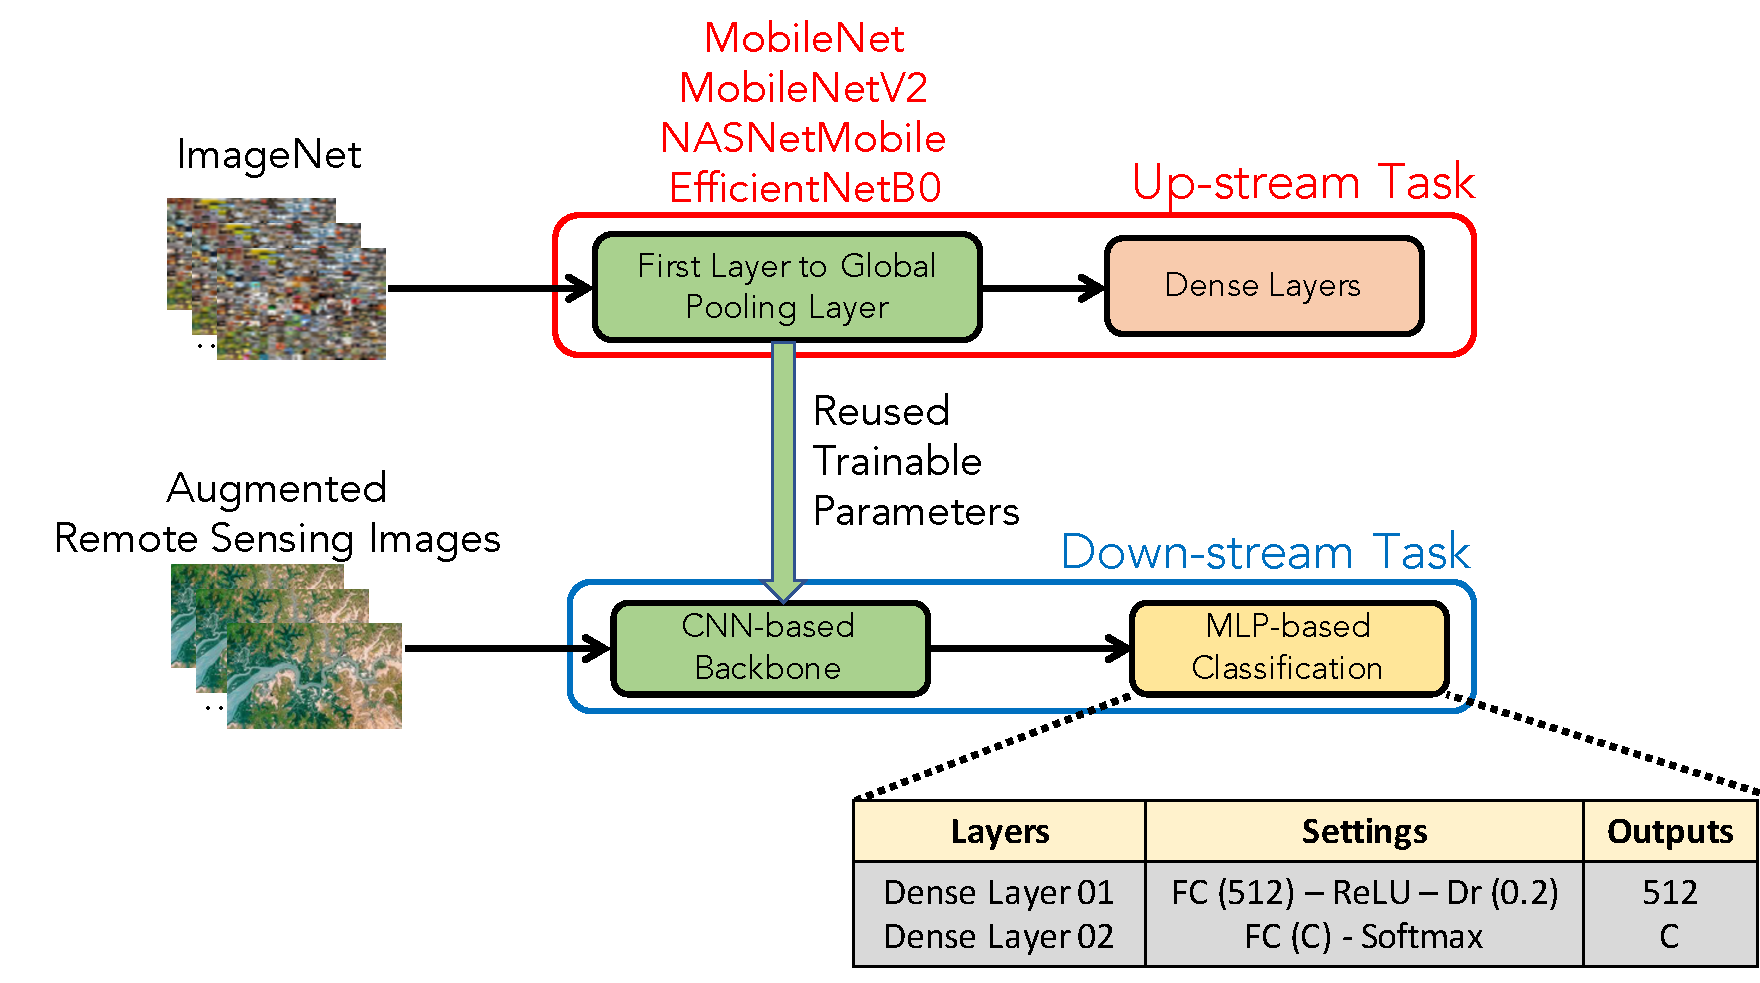
\includegraphics[width=1.0\linewidth]{CAM_trans.pdf}
	\caption{Apply the transfer learning technique for the proposed deep neural network classification}
    \label{fig:CAM_transfer}
\end{figure}

\subsection{Apply attention schemes and explore multiple feature maps to further improve the proposed RSIC system}
\label{app_att}
\begin{figure}[t]
    \centering
    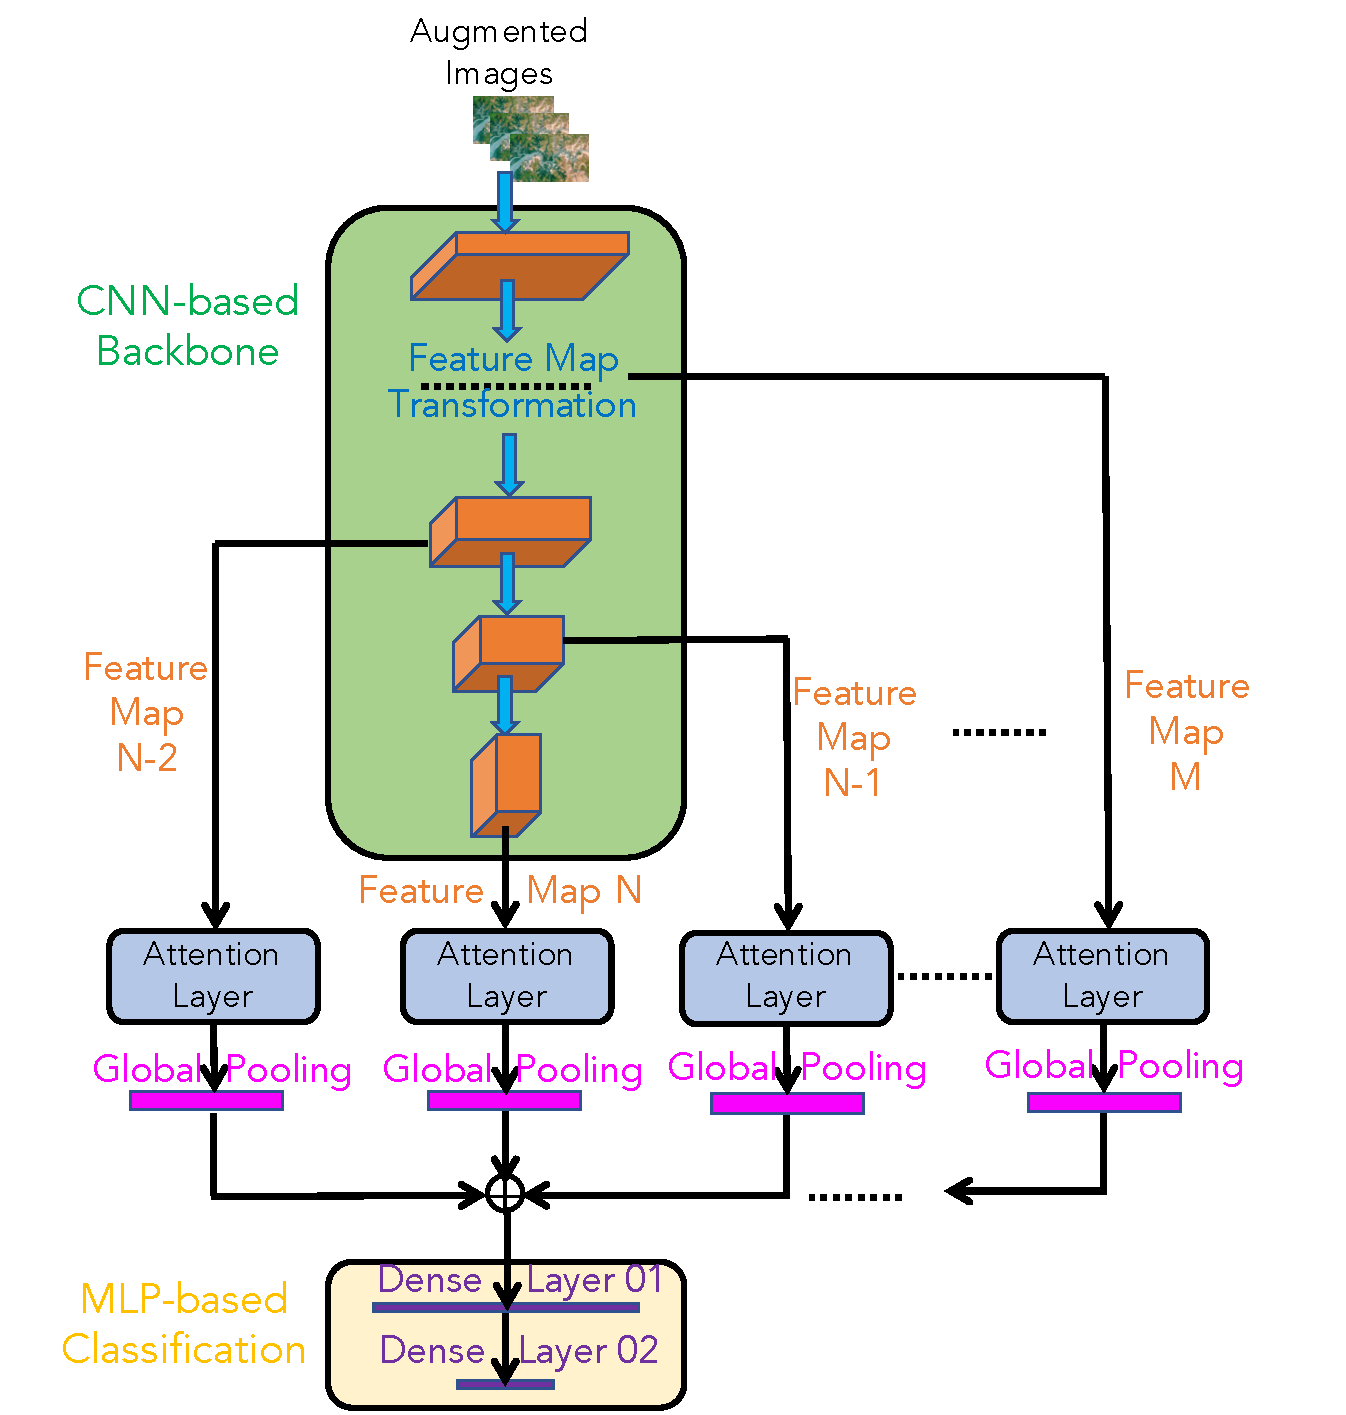
\includegraphics[width=1.0\linewidth]{CAM_att.pdf}
	\caption{Apply attentions schemes to further improve the proposed deep neural network classification}
    \label{fig:CAM_apply_att}
\end{figure}
To further improve the proposed RSIC system, we apply different attention schemes mentioned in Section~\ref{attention} to feature maps extracted from middle layers of the CNN based backbone as shown in Figure~\ref{fig:CAM_apply_att}.
The feature maps are the final outputs of convolutional blocks of the CNN based backbone.
For example, EfficientB0 based backbone presents 7 convolutional blocks, namely block 1 to block 7~\cite{tan2019efficientnet}.
Regarding the attention layer used in Figure~\ref{fig:CAM_apply_att}, we evaluate three types of attention schemes: SE, CBAM, and Multihead attention.
The first two attention layers of SE and CBAM are constructed based on the formulations mentioned in Section~\ref{attention}.
For the Multihead attention scheme, we propose a Multihead attention based layer as shown in Figure~\ref{fig:CAM_pro_att}.
In particular, given an input feature map $\mathbf{X}$ with a size of [W$\times$H$\times$C] where $W$, $H$, and $C$ presents width, height, and channel dimensions, we reduce the size of feature map $\mathbf{X}$ across three dimensions using both max and average pooling layers.
We then generate 3 two-dimensional feature maps, likely matrices of: [W$\times$ H], [H$\times$ C], [W$\times$C]. 
Next we feed all generated matrices into the Multihead attention to obtain attention score matrices. 
Then, we reshape the attention score matrices into the sizes of [W$\times$H$\times$1], [1$\times$H$\times$C],[W$\times$1$\times$C] respectively and element-wise multiply each of them with the input feature map $\mathbf{X}$. 
Finally, we conduct an average of three results of multiplications, generate the output tensor $\mathbf{Y}$ with the size of [W$\times$H$\times$C] which is same size as the input feature map $\mathbf{X}$.
Notably, we set the number of heads to 32 and set the key dimension to 8 for each Multihead attention.
By applying our proposed Multihead attention based layer, both channel feature (feature maps with sizes of [H$\times$ C], [W$\times$C]) and spatial feature (feature map with size of [W$\times$ H]) are focused, which helps the network learn distinct features from the input feature map better.

As SE, CBAM, or our proposed Multihead attention base layers only transforms an input feature map $\mathbf{X}$ to an output feature map $\mathbf{Y}$ and retains the size of the input feature map $\mathbf{X}$, we then apply a global average pooling layer after each attention layer to scale down the feature maps to one-dimensional feature maps, likely vectors.
Finally, these vectors are added together and feed into the MLP-based classifier for classification as shown in Figure~\ref{fig:CAM_transfer}.
  
\begin{figure}[t]
    \centering
    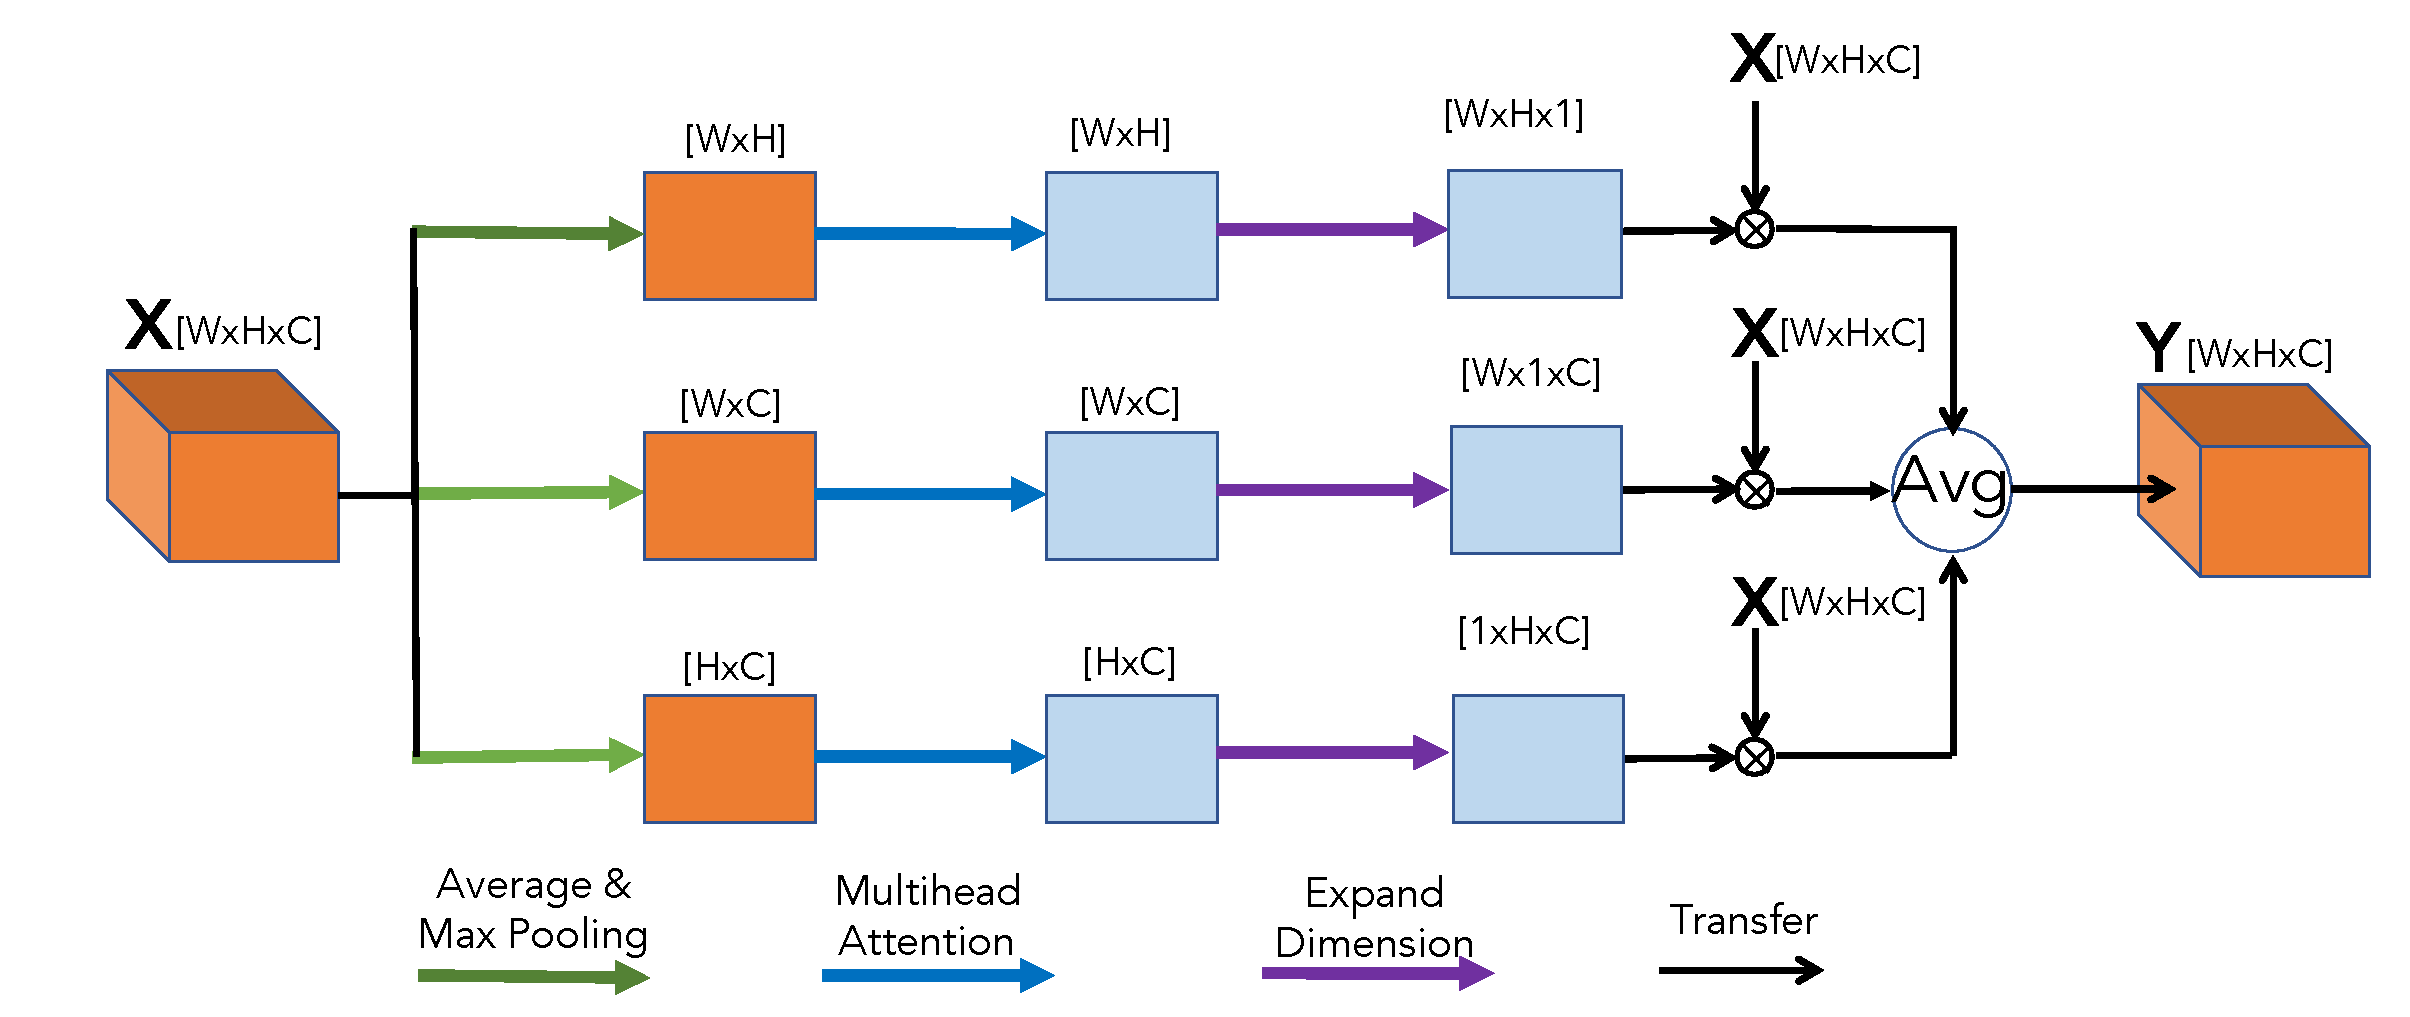
\includegraphics[width=1.0\linewidth]{CAM_pro_att.pdf}
	\caption{Proposed Multihead attention based layer.}
    \label{fig:CAM_pro_att}
\end{figure}

\section{Experimental results and discussion}

\subsection{Dataset}
\label{dataset}

In this paper, we evaluate the benchmark dataset NWPU-RESISC45\cite{nwpu_dataset}.
NWPU-RESISC45 dataset was collected from more than 100 countries and regions in the world, consisting of 31,500 remote sensing images. 
The remote sensing images are separated into 45 scene classes, each of which comprises 700 images in RGB color format with resolution of $256\times256\times3$
To compare with the state-of-the-art systems, we obey the original settings mentioned in~\cite{nwpu_dataset}.
We then split the NWPU-RESISC45 dataset into Training-Testing subsets with two different ratios: 20\%-80\%  and 10\%-90\%, respectively.

\subsection{Evaluation Metrics}
To compare with the state-of-the-art systems, Accuracy (Acc.\%) is used as the main metric, which was proposed in almost benchmark datasets of AID\cite{aid_dataset}, UCM\cite{yang2010bag}, or NWPU-RESISC45\cite{nwpu_dataset}.  

\subsection{Model implementation and settings}
\label{setting}
As the data augmentation method of Mixup~\cite{mixup2} is applied, the ground truth are not in one-hot encoding format. 
We therefore apply Kullback-Leibler divergence (KL) loss~\cite{kl_loss} instead of Entropy loss.
%
\begin{align}
   \label{eq:kl_loss}
   Loss_{KL}(\Theta) = \sum_{n=1}^{N}\mathbf{y}_{n}\log \left\{ \frac{\mathbf{y}_{n}}{\mathbf{\hat{y}}_{n}} \right\}  +  \frac{\lambda}{2}||\Theta||_{2}^{2} \,,
\end{align}
where  \(\Theta\) presents trainable parameters, the constant \(\lambda\) is empirically set to $0.0001$, the batch size $N$ is set to 60, $\mathbf{y_{i}}$ and $\mathbf{\hat{y}_{i}}$ denote expected and predicted results, respectively.
We construct proposed deep learning networks with Tensorflow framework using
Adam~\cite{adam} for optimization.
The training and evaluating processes are conducted on two GPU Titan RTX 24GB.
The training process is stopped after 60 epoches. 
While the first 50 epoches uses the learning rate of 0.0001 and all data augmentation
methods mentioned in Section~\ref{augmentation}, the remaining 10 epochs use the lower learning rate of 0.000001 with only the offline Random Rotation data augmentation method.

\subsection{Experimental results}
%--------------------
\begin{table}[t]
    \caption{Performance comparison among benchmark network architectures, with the transfer learning technique and without attention scheme, on the benchmark NWPU-RESISC45 dataset using 20\%-80\% splitting settings.} 
            	%\vspace{0.2cm}
    \centering
    \scalebox{1.0}{
    \begin{tabular}{|l|c|c|} 
        \hline 
        \textbf{Network}  &\textbf{Accuracy (\%)}        &\textbf{Parameters (M)/} \\
                          &                              &\textbf{Memory (MB)} \\

  	    \hline         
        \textbf{MobileNet} &90.2 &3.7/14.8\\
        \textbf{MobileNetV2} &90.9 &2.9/11.6\\
        \textbf{NASNetMobile}  &91.7 &4.8/19.2\\
        \textbf{EfficientNetB0}  &92.0 &4.6/18.4\\
         \hline 
      \end{tabular}
    }
    %\vspace{-0.3cm}
    \label{table:res01} 
\end{table}
%-------------------
%--------------------
\begin{table}[t]
    \caption{Performance comparison of EfficientB0 with the transfer learning and different attention schemes on the benchmark NWPU-RESISC45 dataset using 20\%-80\% splitting settings.} 
            	%\vspace{0.2cm}
    \centering
    \scalebox{1.0}{
    \begin{tabular}{|l|c|c|c|} 
        \hline 
        \textbf{Attention}  &\textbf{SE} &\textbf{CBAM} &\textbf{Proposed Multihead}   \\
	    \hline         
	            \textbf{Accuracy (\%)}   &92.1  &92.3 &93.8  \\
	            \textbf{Parameters (M)}  &10.4  &6.7  &9.4  \\
  	            \textbf{Memory (MB)}     &41.6  &26.8 &37.6  \\

         \hline 
      \end{tabular}
    }
    %\vspace{-0.3cm}
    \label{table:res02} 
\end{table}
%-------------------

According to the results shown in Table \ref{table:res01}, the proposed RSIC system using the transfer learning technique and EfficientNetB0 and NASNetMobile based architectures are competitive and outperform MobileNet and MobileNetV2.
As EfficientNetB0 accuracy (92.0\%) is not only better than NASNetMobile (91.7\%) but EfficientNetB0 footprint (4.6 M/18.8 MB) is also smaller than NASNetMobile (4.8 M/19.2 MB), we select EfficientNetB0 architecture for further experiments.

Given EfficientNetB0 backbone, we evaluate our proposed RSIC system applying three types of attention layers: SE, CBAM, and the proposed Multihead attention.
In this experiment, only the feature maps which are extracted from the final three convolutional blocks (block 5 to block 7) in the EfficientNetB0 backbone are used. 
As Table~\ref{table:res02} shows, applying attention layers helps to improve the system performance by 0.1\%, 0.3\%, and 1.8\% with SE, CBAM, and the proposed Multihead attention, respectively.

As the proposed Multihead attention layer outperforms SE and CBAM layers, we then evaluate the proposed Multihead attention with a different number of feature maps.
As the results are shown in Table~\ref{table:res03}, using three feature maps still achieves the best performance.
Regarding the model complexity, using the proposed Multihead attention layer with three feature maps increases the model footprint from 4.6 M to 9.4 M, which leads to occupy from 18.4 MB to 37.6 MB memory (i.e. 1 trainable parameter is presented by 32 bit in floating point format).
To meet the constrain of maximum memory occupation of 20 MB on application device, we apply the quantization technique which helps to reduce the model complexity to 9.4 MB (i.e. The quantization technique helps to quantize a 32-bit floating point to 8-bit integer, then reduce the model footprint to 1/4 of the original footprint).
Notably, although the pruning techniques can help to significantly reduce a deep learning model to 1/10 of the original size~\cite{pajusco2020lightweight}, pruning parameters considered as zero still occupy the memorize of edge devices and cost the same computation as the non-pruning parameters.
Therefore, the pruning technique is not applied in this paper.

By using EfficientNetB0 as CNN-based backbone, the transfer learning, the proposed Multihead attention layer for three feature maps and the quantization technique, we achieve a low-complexity RISC model (9.4 M trainable parameters and 9.4 MB memory occupation).
We evaluate this model on NWPU-RESISC45 with two splitting settings as mentioned in Section~\ref{dataset} and compare with the state-of-the-art systems.
As Table \ref{table:res_11} shows, we can see that our results are very competitive compared with the state-of-the-art systems.
We achieve accuracy scores of 91.0\% and 93.8\% with training proportions of 10\% and 20\% respectively.
Compared with the system also using EfficientNetB0 in~\cite{sota_05}, our proposed RSIC not only outperforms but also presents a lower model footprint.
Our proposed system performs lower than 2\% compared with the best model using a Transformer based architecture~\cite{sota_13}. 
However, our model presents a significantly low footprint (9.4 M / 9.4 MB) compared with the best Transformer based model (46.3 M / 185.2 MB).
%--------------------
\begin{table}[t]
    \caption{Performance (Acc.\%) of EfficientNetB0 with the proposed Multihead attention applied for feature maps extracted from different convolutional blocks on the benchmark NWPU-RESISC45 dataset using 20\%-80\% splitting settings.} 
            	%\vspace{0.2cm}
    \centering
    \scalebox{1.0}{
    \begin{tabular}{|c|c|c|} 
        \hline 
        \textbf{Convolutional Blocks}  &\textbf{Accuracy (\%)}        &\textbf{Parameters (M)/} \\
                                      &                              &\textbf{Memory (MB)} \\
  	    \hline         
        \textbf{Block 7}       &93.1 &6.0/24\\
        \textbf{Blocks 6 to 7}  &93.0 &7.5/30\\
        \textbf{Blocks 5 to 7}  &93.8 &9.4/37.6\\
        \textbf{Blocks 4 to 7}  &92.8 &11.2/44.8\\
        \textbf{Blocks 3 to 7}  &92.5 &13.3/53.2\\
         \hline 
      \end{tabular}
    }
    %\vspace{-0.3cm}
    \label{table:res03} 
\end{table}
%-------------------
%--------------------
\begin{table}[t]
    \caption{Performance (Acc.\%) comparison to the state-of-the-art systems on the benchmark NWPU-RESISC45 dataset with two splitting settings.} 
            	%\vspace{0.2cm}
    \centering
    \scalebox{0.9}{

    \begin{tabular}{|l|c|c|} 
        \hline 
\textbf{Methods}                                       &\textbf{10\% training} &\textbf{20\% training} \\
	    \hline         
MG-CAP (Log-E) (55.99 M)~\cite{sota_01}                &89.4                   &91.7 \\ 
MG-CAP (Bilinear) (55.99 M)~\cite{sota_01}             &89.4                   &93.0 \\
MG-CAP (Sqrt-E) (55.99 M)~\cite{sota_01}               &90.8                   &93.0 \\ 
EfficientNet-B0-aux ($\approx 5.3 M$)~\cite{sota_05}   &90.0                   &92.9  \\
EfficientNet-B3-aux ($\approx 13 M$)~\cite{sota_05}    &91.1                   &93.8  \\
VGG-16 + MTL ($\approx$ 138.4 M)~\cite{sota_11}        &-                      &91.5 \\ 
ResNeXt-50 + MTL ($\approx$ 25 M)~\cite{sota_11}       &-                      &93.8 \\
ResNeXt-101 + MTL ($\approx$ 88.79 M)~\cite{sota_11}   &91.9                   &94.2 \\
SE-MDPMNet (5.17 M)~\cite{sota_10}                     &91.8                   &94.1 \\
LGRIN (4.63 M)~\cite{sota_12}                          &91.9                   &94.4 \\
Transformer (46.3 M)~\cite{sota_13}                    &93.1                   &95.6 \\ 
        \hline 
        
\textbf{Our systems(9.4 M/9.4 MB)}                           &\textbf{91.0}          &\textbf{93.8} \\
         \hline 
      \end{tabular}
    }
    %\vspace{-0.3cm}
    \label{table:res_11} 
\end{table}
%-------------------

%%--------------------
%\begin{table*}[t]
%    \caption{Performance (Acc.\%) comparison to the state-of-the-art systems on the benchmark UMC, AID, and NWPU-RESISC45 datasets with the different splitting settings.} 
%            	%\vspace{0.2cm}
%    \centering
%    \scalebox{1.0}{
%
%    \begin{tabular}{|l||c|c||c|c||c|c|} 
%        \hline 
%\textbf{Methods}                     &\textbf{50\% training} &\textbf{80\% training} &\textbf{20\% training} &\textbf{50\% training} &\textbf{10\% training} &\textbf{20\% training} \\
%	    \hline         
%MG-CAP (Log-E) (55.99 M)~\cite{sota_01}        &-                      &98.4                   &90.1                   &94.8                   &89.4                   &91.7 \\ 
%MG-CAP (Bilinear) (55.99 M)~\cite{sota_01}     &-                      &98.6                   &92.1                   &95.1                   &89.4                   &93.0 \\
%MG-CAP (Sqrt-E) (55.99 M)~\cite{sota_01}       &-                      &99.0                   &93.3                   &96.1                   &90.8                   &93.0 \\ 
%EfficientNet-B0-aux ($\approx 5.3 M$)~\cite{sota_05}   &98.0                   &99.0                   &93.7                   &96.1                   &90.0                   &92.9  \\
%EfficientNet-B3-aux ($\approx 13 M$)~\cite{sota_05}   &98.2                   &99.0                   &94.2                   &96.5                   &91.1                   &93.8  \\
%VGG-16 + MTL ($\approx$ 138.4 M)~\cite{sota_11}          &-                      &98.3                   &-                      &94.7                   &-                      &91.5 \\ 
%ResNeXt-50 + MTL ($\approx$ 25 M)~\cite{sota_11}      &-                      &99.0                   &-                      &96.5                   &-                      &93.8 \\
%ResNeXt-101 + MTL ($\approx$ 88.79 M)~\cite{sota_11}     &-                      &99.1                   &94.0                   &96.9                   &91.9                   &94.2 \\
%SE-MDPMNet (5.17 M)~\cite{sota_10}            &98.5                   &99.0                   &94.7                   &97.1                   &91.8                   &94.1 \\
%LGRIN (4.63 M)~\cite{sota_12}           &98.6                   &99.0                   &94.7                   &97.6                   &91.9                   &94.4 \\
%Transformer (46.3 M)~\cite{sota_13}           &98.7                   &99.5                   &95.5                   &98.5                   &93.1                   &95.6 \\ 
%        \hline 
%\textbf{Our systems (2.4 M)}                 &\textbf{93.5}          &\textbf{96.0}          &\textbf{91.0}          &\textbf{94.0}          &\textbf{91.0}          &\textbf{93.8} \\
%         \hline 
%      \end{tabular}
%    }
%    %\vspace{-0.3cm}
%    \label{table:res_11} 
%\end{table*}
%%-------------------
\section{Conclusion}
%
This paper has presented a deep learning based model for remote sensing image classification (RSIC).
By conducting extensive experiments, we indicate that applying multiple techniques of transfer learning, Multihead attention on  multiple feature maps, and quantization to EfficientNetB0 based network architecture helps to achieve a high-performance and low-complexity RSIC system. 
The experimental results prove our proposed RSIC system competitive to the state-of-the-art systems and potential to apply on a wide range of edge devices.

\begin{acks}
    We would like to thank Ho Chi Minh City University of Technology (HCMUT), Vietnam National University Ho Chi Minh City (VNU-HCM) for the support of time and facilities for this study.
\end{acks}

%----------------------- CITATION
%% The next two lines define the bibliography style to be used, and
%% the bibliography file.
\bibliographystyle{ACM-Reference-Format}
\bibliography{sample-base}


\end{document}
\endinput
%%
%% End of file `sample-sigconf.tex'.
